\documentclass[a4paper]{article}

%Tutti gli usepackage vanno qui

\usepackage{geometry}
\usepackage[italian]{babel}
\usepackage[utf8]{inputenc}
\usepackage[T1]{fontenc}
\usepackage{tgschola}
%\usepackage{tgbonum}
\usepackage{tabularx}
\usepackage{longtable}
\usepackage{hyperref}
\usepackage{enumitem}
\usepackage[toc]{appendix}
\hypersetup{
	colorlinks=true,
	linkcolor=black,
	filecolor=magenta,      
	urlcolor=blue,
}
% Numerazione figure 
\let\counterwithout\relax
\let\counterwithin\relax
\usepackage{chngcntr}

\counterwithin{table}{subsection}
\counterwithin{figure}{subsection}

\usepackage[bottom]{footmisc}
\usepackage{fancyhdr}
\setcounter{secnumdepth}{4}
\usepackage{amsmath, amssymb}
\usepackage{array}
\usepackage{graphicx}

\usepackage{ifthen}

%\usepackage{float}
\usepackage{layouts}
\usepackage{url}
\usepackage{comment}
\usepackage{float}
\usepackage{eurosym}

\usepackage{lastpage}
\usepackage{layouts}
\usepackage{float}
\usepackage{eurosym}

%Comandi di impaginazione uguale per tutti i documenti
\pagestyle{fancy}
\lhead{
\includegraphics[scale=0.04]{../../../../latex/images/logoTWM.png}}
%Titolo del documento
\rhead{\doctitle{}}
%\rfoot{\thepage}
\cfoot{Pagina \thepage\ di \pageref{LastPage}}
\setlength{\headheight}{35pt}
\setcounter{tocdepth}{5}
\setcounter{secnumdepth}{5}
\renewcommand{\footrulewidth}{0.4pt}

% multirow per tabelle
\usepackage{multirow}

% Permette tabelle su più pagine
%\usepackage{longtable}


% colore di sfondo per le celle
\usepackage[table]{xcolor}

%COMANDI TABELLE
\newcommand{\rowcolorhead}{\rowcolor[HTML]{9b240a}} %intestazione 
% check for missing commands
\newcommand{\headertitle}[1]{\textbf{\color{white}#1}} %titolo colonna
\definecolor{pari}{HTML}{FFDBCB}
\definecolor{dispari}{HTML}{F1F7FD}

% comandi glossario
\newcommand{\glo}{$_{G}$}
\newcommand{\glosp}{$_{G}$ }


%label custom
\makeatletter
\newcommand{\uclabel}[2]{%
	\protected@write \@auxout {}{\string \newlabel {#1}{{#2}{\thepage}{#2}{#1}{}} }%
	\hypertarget{#1}{#2}
}
\makeatother

%riportare pezzi di codice
\definecolor{codegray}{gray}{0.9}
\newcommand{\code}[1]{\colorbox{codegray}{\texttt{#1}}}



% Configurazione della pagina iniziale
\newcommand{\doctitle}{Norme di Progetto}
\newcommand{\docdate}{ } % lasciare vuoto (uno carattere di spazio) per i documenti che non sono verbali, così non viene scritta la data
\newcommand{\rev}{3.0.1}
\newcommand{\stato}{Non Approvato}
\newcommand{\uso}{Interno}
\newcommand{\approv}{--De Renzis Simone}
\newcommand{\red}{Greggio Nicolò\\& Tessari Andrea}
\newcommand{\ver}{Zuccolo Giada\\& Crivellari Alberto}
\newcommand{\dest}{Three Way Milkshake\\ Prof. Vardanega Tullio\\ Prof.
 Cardin Riccardo}
\newcommand{\describedoc}{Questo documento contiene tutte le norme di progetto\textsubscript{G}, definite inizialmente o aggiunte in seguito, viene quindi aggiornato per incrementi successivi.}



 % modifica questo file
\makeindex

\usepackage{hyperref}


\usepackage[toc,acronym]{glossaries}
\makeglossaries

\newglossaryentry{wiki}{name={wiki}, plural={wikis},%
	description={Termine di origine hawaiana che significa veloce, con cui si identifica un tipo di sito internet che permette la creazione e la modifica di pagine multimediali attraverso un'interfaccia semplice}}

\newglossaryentry{vmodel}{name={Modello a V},%
	description={Modello che illustra le relazioni tra ogni fase del ciclo di vita del software con la relativa fase di testing ad essa associata}}

\newglossaryentry{usecase}{name={caso d'uso}, plural={casi d'uso},%
	description={Un caso d'uso è un insieme di \glspl{scenario} che hanno in comune uno scopo finale (obiettivo) per un utente (\gls{attore})}}

\newglossaryentry{techbase}{name={technology baseline},%
	description={Motiva le tecnologie, i framework, e le librerie selezionate per la realizzazione del prodotto. Ne dimostra adeguatezza e fattibilità, tramite un proof of concept coerente con gli obiettivi}}

\newglossaryentry{task}{name={task}, plural={tasks},%
	description={Nel contesto del capitolato, con questo termine si identifica un compito da svolgere da parte di un unità (muletto) che consiste nel raggiungere un \acrshort{POI} e caricare o scaricare la merce}}

\newglossaryentry{stakeholder}{name={stakeholder}, plural={stakeholders},%
	description={Tutti coloro che a vario titolo hanno influenza sul prodotto e sul progetto. Sono stakeholders il committente, il proponente, gli utenti, il team di sviluppo}}

\newglossaryentry{sistematico}{name={sistematico},%
	description={Modo di lavorare metodico e rigoroso, che conosce, usa ed evolve le best practice di dominio}}

\newglossaryentry{shell}{name={shell},%
	description={Interprete dei comandi}}

\newglossaryentry{security}{name={security},%
	description={Non vulnerabilità rispetto a intrusioni}}

\newglossaryentry{scenario}{name={scenario}, plural={scenari},%
	description={Nell'ambito dello sviluppo software, sequenza di passi che descrive l'interazione tra l'\gls{attore} e il sistema, e le elaborazioni necessarie per soddisfare la richiesta dell'\gls{attore}}}

\newglossaryentry{safety}{name={safety},%
	description={Sicurezza rispetto a malfunzionamenti}}

\newglossaryentry{risorsa}{name={risorsa}, plural={risorse},%
	description={Mezzo o capacità disponibile, nello sviluppo software ad esempio le persone, il tempo, il denaro, gli strumenti necessari allo sviluppo del progetto. Le attività di progetto consumano le risorse disponibili}}

\newglossaryentry{revisione}{name={revisione}, plural={revisioni},%
	description={Esame o controllo, per lo più periodico, inteso a verificare il grado dell'efficienza, della funzionalità, della corrispondenza a determinati requisiti. Nell'ambito del corso di Ingegneria del Software, la revisione di avanzamento identifica il momento in cui il team consegna e presenta gli artefatti sviluppati durante il periodo appena trascorso}}

\newglossaryentry{requisito}{name={requisito}, plural={requisiti},%
	description={Esistono due interpretazioni principali di un requisito \begin{itemize}\item dal lato del bisogno(ovvero il cliente/utente) è la capacità necessaria a un utente per risolvere un problema o raggiungere un obiettivo\item dal lato della soluzione (ovvero lo sviluppatore) è la capacità che deve essere posseduta (o condizione che deve essere soddisfatta) da un sistema per adempiere a un obbligo \end{itemize}}}

\newglossaryentry{repository}{name={repository},%
	description={Posizione di archiviazione per pacchetti software}}

\newglossaryentry{quantificabile}{name={quantificabile},%
	description={Che permette di misurare l'efficienza e l'efficacia del suo agire}}

\newglossaryentry{proofconcept}{name={proof of concept},%
	description={Dimostratore eseguibile. Il suo codice può (ma non deve) essere usa-e-getta}}

\newglossaryentry{progetto}{name={progetto}, plural={progetti},%
	description={Insieme di attività che devono raggiungere determinati obiettivi a partire da determinate specifiche; hanno una data d'inizio e una data di fine fissate, dispongono di risorse limitate e consumano tali risorse nel loro svolgersi}}

\newglossaryentry{prodbase}{name={product baseline},%
	description={Illustra la baseline architetturale del prodotto, coerente con la \acrshort{tb}. Rappresenta il design definitivo}}

\newglossaryentry{precondizione}{name={precondizione}, plural={precondizioni},%
	description={Condizioni che devono essere soddisfatte affinché si verifichino determinati eventi successivi}}

\newglossaryentry{postcondizione}{name={postcondizione}, plural={postcondizioni},%
	description={Condizioni che devono verificarsi dopo determinati eventi}}

\newglossaryentry{planimetria}{name={planimetria}, plural={planimetrie},%
	description={Rappresentazione in piano del magazzino che ne evidenzia le caratteristiche (aree non transitabili, zone di percorrenza, punti di interesse)}}

\newglossaryentry{periodo}{name={periodo}, plural={periodi},%
	description={Nel contesto del documento, l'intervallo di tempo che intercorre tra due revisioni successive}}

\newglossaryentry{percorrenza}{name={percorrenza}, plural={percorrenze},%
	description={Nel contesto del capitolato, i vincoli relativi alle zone transitabili: \begin{itemize} \item sensi di marcia \item numero massimo di unità che vi possono transitare \end{itemize}}}

\newglossaryentry{modellosviluppo}{name={modello di sviluppo},%
	description={Principio teorico che indica il metodo da seguire nel progettare e nello scrivere un programma. Esistono tre principali modelli di sviluppo, ossia sequenziale, \gls{incrementale} ed evolutivo.}}

\newglossaryentry{milestone}{name={milestone},%
	description={Pietra miliare, istante temporale su cui si misura l'avanzamento del progetto. Viene fissata nel futuro per stabilire un avanzamento atteso. Una buona milestone è delimitata per ampiezza ed ambizioni, misurabile in termini di tempo e impegno necessario per raggiungerla, traducibile in compiti assegnabili ai membri del team e coerente con le scadenze del progetto}}

\newglossaryentry{kanban}{name={kanban},%
	description={Framework usato per implementare modelli di sviluppo Agili e DevOps. Richiede comunicazione in tempo reale tra i componenti de team e totale trasparenza. I work item vengono visualizzati su una Kanban Board, permettendo ai membri del team di vedere lo stato di ogni attività in ogni momento. Per maggiori dettagli \url{https://www.atlassian.com/agile/kanban/kanban-vs-scrum}}}

\newglossaryentry{incrementale}{name={incrementale},%
	description={Che procede per incrementi, ossia migliorie che, partendo da un impianto base, portano al raggiungimento dell'obiettivo producendo valore e limitando al massimo la regressione a stati già attraversati}}

\newglossaryentry{gitpush}{name={git-push},%
	description={Azione di git che permette di caricare le proprie modifiche locali sul server remoto condiviso del repository}}

\newglossaryentry{gitpull}{name={pull},%
	description={Comando di \gls{git} che permette di aggiornare il proprio \acrshort{repo} locale con i cambiamenti remoti}}

\newglossaryentry{git}{name={git},%
	description={Sistema di controllo del versionamento distribuito}}

\newglossaryentry{gitcommit}{name={commit}, plural={commits},%
	description={Comando di \gls{git} che permette di salvare e versionare le modifiche attuate ai file in locale}}

\newglossaryentry{gantt}{name={Gantt},%
	description={Diagramma per la pianificazione di un progetto. Esplicita le attività volte al suo svolgimento e per ognuna ne identifica data di inizio e di fine a seconda delle stime effettuate. Facilità la visualizzazione delle connessioni tra le attività e lo stato di avanzamento del progetto}}

\newglossaryentry{form}{name={form},%
	description={Interfaccia di un programma che consente a un utente di inserire e inviare uno o più dati}}

\newglossaryentry{fase}{name={fase}, plural={fasi},%
	description={Segmento temporale contiguo che che presuppone uno stazionamento in uno stato o in una transizione di ciclo di vita}}

\newglossaryentry{efficienza}{name={efficienza},%
	description={Misura dell'abilità di raggiungere l'obiettivo impiegando le risorse in maniera ottimale}}

\newglossaryentry{efficacia}{name={efficacia},%
	description={Misura della capacità di raggiungere l'obiettivo prefissato}}

\newglossaryentry{disciplinato}{name={disciplinato},%
	description={Che segue le regole che si è dato}}

\newglossaryentry{designpattern}{name={design pattern}, plural={design patterns},%
	description={Soluzione progettuale generale ad un problema ricorrente}}

\newglossaryentry{cruscotto}{name={cruscotto}, plural={cruscotti},%
	description={Interfaccia utente grafica che fornisce viste indicatori chiave di prestazione rilevanti per un particolare obiettivo o processo aziendale}}

\newglossaryentry{combobox}{name={combobox},%
	description={Controllo grafico (widget) che permette all'utente di effettuare una scelta scrivendola in una casella di testo o selezionandola da un elenco}}

\newglossaryentry{capitolato}{name={capitolato}, plural={capitolati},%
	description={Documento tecnico redatto dal cliente in cui vengono specificati i vincoli contrattuali (prezzo e scadenze) per lo sviluppo di un determinato prodotto software. Viene presentato in un bando d'appalto per trovare qualcuno che possa svolgere il lavoro richiesto}}

\newglossaryentry{bug}{name={bug},%
	description={Problema che porta al malfunzionamento del software, per esempio producendo un risultato inatteso o errato, tipicamente dovuto a un errore nella scrittura del codice sorgente di un programma}}

\newglossaryentry{bestpractice}{name={best practice}, plural={best practices},%
	description={Modo di fare noto, che abbia mostrato di garantire i migliori risultati in circostanze note e specifiche}}

\newglossaryentry{bash}{name={bash},%
	description={G:bash:bash:X:\gls{shell} Unix ed un linguaggio interpretato scritto da Brian Fox per il progetto GNU come sostituto del software gratuito per la shell Bourne}}

\newglossaryentry{baseline}{name={baseline},%
	description={Istantanea dello stato di avanzamento del progetto. Misura i risultati ottenuti e li fissa in una versione consolidata del prodotto. Può essere associata ad un rifermento temporale (\gls{milestone})}}

\newglossaryentry{attore}{name={attore}, plural={attori},%
	description={Ruolo interpretato da un utente (persona o sistema esterno) nei confronti del sistema. \begin{itemize} \item \textbf{attore primario}: attore richiede l'assistenza del sistema \item \textbf{attore secondario}: attore di cui è il sistema stesso a richiedere l'intervento \end{itemize}}}

\newglossaryentry{attivita}{name={attività},%
	description={Insieme di una o più azioni il cui completamento porta ad un avanzamento nel complesso}}

\newglossaryentry{artefatto}{name={artefatto}, plural={artefatti},%
	description={Sottoprodotto che viene realizzato durante lo sviluppo software. Sono artefatti i casi d'uso, i diagrammi delle classi, i modelli UML, il codice sorgente e la documentazione varia, che aiutano a descrivere la funzione, l'architettura e la progettazione del software}}

\newglossaryentry{agile}{name={agile},%
	description={Approccio stutturato e iterativo alla gestione dei progetti e alla sviluppo di software. Riconosce la volatilità dello sviluppo del prodotto e propone un metodo per permettere ai team di rispondere in maniera rapida a cambiamenti non pianificati e di produrre valore fin dalle prime iterazioni. Per maggiori dettagli \url{https://www.atlassian.com/agile/kanban/kanban-vs-scrum}}}

\newacronym{vcs}{VCS}{Version Control System}

\newacronym{uml}{UML}{Unified Modeling Language}

\newacronym{tb}{TB}{\gls{techbase}}

\newacronym{spa}{spa}{X}

\newacronym{rest}{REST}{REpresentational State Transfer}

\newacronym{repo}{repo}{\gls{repository}}

\newacronym{ram}{RAM}{Random Access Memory}

\newacronym{portacs}{PORTACS}{\acrshort{POI} Oriented Real Time Anti Collision System}

\newacronym{POI}{POI}{Point Of Interest}

\newacronym{poc}{PoC}{Proof of Concept}

\newacronym{pb}{PB}{\gls{prodbase}}

\newacronym{jit}{JiT}{Just in Time}

\newacronym{faas}{FaaS}{Functions as a Service}

\newacronym{eg}{e.g.}{Example given, si usa per indicare che ciò che segue è un esempio}

\newacronym{cpu}{CPU}{Central Processing Unit}

\newacronym{cms}{CMS}{Content Management System}

\newacronym{baas}{BaaS}{Backend as a Service}

\newacronym{api}{API}{Application Programming Interface}


\begin{document}
	\thispagestyle{empty}
\begin{titlepage}
	\begin{center}
		
		
\includegraphics[scale = 0.17]{../../../../latex/images/logoTWM.png}\\[0.7cm]
		

		\noindent\rule{\textwidth}{1pt} \\[0.4cm]
		\Huge \textbf{\doctitle} \\[0.1cm]
		\ifthenelse{\equal{\docdate}{ }}{ }{ \huge \textbf{\docdate} \\[0.1cm] }
		
		\noindent\rule{\textwidth}{1pt}\\[0.7cm]
		
		\large \textbf{Three Way Milkshake - Progetto "PORTACS"} \\[0.4cm] 
                \texttt{threewaymilkshake@gmail.com} \\[0.4cm]
                
		
        
        
        \large

        \begin{tabular}{r|l}
                        \textbf{Versione} & \rev{} \\
                        \textbf{Stato} & \stato{} \\
                        \textbf{Uso} & \uso{} \\                         
                        \textbf{Approvazione} & \approv{} \\                      
                        \textbf{Redazione} & \red{} \\ 
                        \textbf{Verifica} &  \ver{} \\                         
                        \textbf{Destinatari} & \parbox[t]{5cm}{ \dest{} }
                \end{tabular} 
                \\[0.3cm]
                \large \textbf{Descrizione} \\ \describedoc{} 
               

	\end{center}
\end{titlepage}
	\pagebreak	
	
	% Registro delle modifiche
	\section*{Registro delle modifiche}

\newcommand{\changelogTable}[1]{
	
	
	\renewcommand{\arraystretch}{1.5}
	\rowcolors{2}{pari}{dispari}
	\begin{longtable}{ 
			>{\centering}p{0.07\textwidth} 
			>{}p{0.21\textwidth}
			>{\centering}p{0.17\textwidth}
			>{\centering}p{0.13\textwidth} 
			>{\centering}p{0.17\textwidth} 
			>{\centering}p{0.13\textwidth} }
		\rowcolorhead
		\headertitle{Vers.} &
		\centering \headertitle{Descrizione} &	
		\headertitle{Redazione} &
		\headertitle{Data red.} & 
		\headertitle{Verifica} &
		\headertitle{Data ver.}
		\endfirsthead	
		\endhead
		
		#1
		
	\end{longtable}
	\vspace{-2em}
	
}


\newcommand{\approvingTable}[1]{ 
	
	
	\renewcommand{\arraystretch}{1.5}
	\rowcolors{2}{pari}{dispari}
	\begin{longtable}{ 
			>{\centering}p{0.07\textwidth} 
			>{\centering}p{0.415\textwidth}
			>{\centering}p{0.13\textwidth}
			>{\centering}p{0.322\textwidth}  }
		\rowcolorhead
		\headertitle{Vers.} &
		\centering \headertitle{Descrizione} &	
		\headertitle{Data appr.} &
		\headertitle{Approvazione}
		\endfirsthead	
		\endhead
		
		#1
		
	\end{longtable}
	\vspace{-2em}
	
}
	\changelogTable{
	3.5.0 & Incremento appendice \S\ A e B & Crivellari Alberto & 2021-04-26 & -- & --
	3.4.0 & Rimossa appendice \S\ D & Crivellari Alberto & 2021-04-01 & -- & --
	\tabularnewline
	3.3.0 & Modifica sezioni \S\ 2 e \S\ 3 & Crivellari Alberto & 2021-04-01 & -- & --
	\tabularnewline
	3.2.0 & Modifica appendice \S\ B & Zuccolo Giada & 2021-03-31 & -- & --
\tabularnewline
	3.1.0 & Aggiornamento appendice \S\ C & Crivellari Alberto & 2021-03-20 & -- & --
}

\approvingTable{
    3.0.0 & Approvazione del documento & 2021-03-08 & Zuccolo Giada
}

\changelogTable{
    2.1.0 & Aggiornamento sezioni \S\ 4 e 5 & Crivellari Alberto & 2021-03-08 & Chiarello Sofia & 2021-03-08
}

\approvingTable{
    2.0.0 & Approvazione del documento & 2021-02-22 & De Renzis Simone
}

\changelogTable{
1.3.0 & Completamento stesura appendice \S\ D e \S\ B & Crivellari Alberto & 2021-02-12 & Greggio Nicolò & 2021-02-19
\tabularnewline
1.2.1 & Completamento stesura sezione \S\ 2 e \S\ 3 & Chiarello Sofia & 2021-02-11 & Tessari Andrea & 2021-02-13
\tabularnewline
1.2.0 & Stesura sezione \S\ 3 e appendice \S\ C & Chiarello Sofia & 2021-02-09 & Tessari Andrea & 2021-02-12
\tabularnewline
1.1.0 & Stesura sezione \S\ 2 & Chiarello Sofia & 2021-02-08 & Tessari Andrea & 2021-02-13
}

\approvingTable{
	1.0.0 & Approvazione del documento & 2021-01-10 & De Renzis Simone
}

\changelogTable{
0.5.1 & Aggiunta tabelle a sezione \S 4 e \S5 & Crivellari Alberto & 2021-01-08 & Greggio Nicolò & 2021-01-10
\tabularnewline
0.5.0 & Redazione sezione \S 5 & Crivellari Alberto & 2020-12-07 & Greggio Nicolò & 2021-01-10
\tabularnewline
0.4.0 & Redazione sezione \S 4 & Crivellari Alberto & 2020-12-06 & Greggio Nicolò & 2021-01-10
\tabularnewline
0.3.2 & Modifiche sezione \S 1 & Crivellari Alberto & 2020-12-30 & Greggio Nicolò & 2021-01-10
\tabularnewline
0.3.1 & Tabelle sezione \S 3 & Crivellari Alberto & 2020-12-29 & Greggio Nicolò & 2021-01-10
\tabularnewline
0.3.0 & Redazione sezione \S 3 & Tessari Andrea & 2020-12-28 & Greggio Nicolò & 2021-01-10
\tabularnewline
0.2.1 & Tabelle sezione \S 2 & Crivellari Alberto & 2020-12-20 &  Greggio Nicolò & 2021-01-09
\tabularnewline
0.2.0 & Redazione sezione \S 2 & Crivellari Alberto & 2020-12-19 & Greggio Nicolò & 2021-01-09
\tabularnewline
0.1.1 & Modifiche sezione \S 1  & Crivellari Alberto & 2020-12-18 & Greggio Nicolò & 2021-01-09
\tabularnewline
0.1.0 & Redazione sezione \S 1 & Crivellari Alberto & 2020-12-16 & Greggio Nicolò & 2021-01-09
\tabularnewline
0.0.1 & Strutturazione del documento & Tessari Andrea & 2020-12-15 & Greggio Nicolò & 2021-01-09
}


 % modifica questo file       
	\end{longtable}
	\pagebreak
		
	% indice
	\tableofcontents	
	\pagebreak
	
	% indice delle figure
	\listoffigures
	\pagebreak
	
	% indice delle tabelle
	\listoftables
	\pagebreak
		
	% contenuto del documento, ogni sezione in un file
	\section{Introduzione}
\subsection{Scopo del documento}
    Questo documento ha lo scopo di fissare e definire tutte le regole, convenzioni e buone pratiche utili a formare un way of working condiviso alla base da tutti i componenti del gruppo per assicurare una collaborazione efficiente ed efficace. Si discuteranno inoltre i vari strumenti che verranno adottati per facilitare lo sviluppo del progetto\textsubscript{G} e per promuovere un'organizzazione adeguata.
    Si ritiene inoltre che la definizione ed il mantenimento per incremento di un documento condiviso all'interno del gruppo di lavoro, che definisca e raccolga quanto descritto in maniera formale e centralizzata, possa favorire, in un contesto dove i membri possano variare, l'inserimento di nuovi componenti facilitandone l'ambientamento. Pur non essendo questo il contesto di lavoro attuale, è comunque una buona pratica da sperimentare e consolidare.

\subsection{Scopo del prodotto}
Il capitolato\textsubscript{G} C5 propone un progetto\textsubscript{G} in cui viene richiesto lo sviluppo di un software per il monitoraggio in tempo reale di unità che si muovono in uno spazio definito. All'interno di questo spazio, creato dall'utente per riprodurre le caratteristiche di un ambiente reale, le unità dovranno essere in grado di circolare in autonomia, o sotto il controllo dell'utente, per raggiungere dei punti di interesse posti nella mappa.  La circolazione è sottoposta a vincoli di viabilità e ad ostacoli propri della topologia dell'ambiente, deve evitare le collisioni con le altre unità e prevedere la gestione di situazioni critiche nel traffico.

\subsection{Termini, abbreviazioni ed altri documenti}
    Tutti i termini che necessitano di una spiegazione, per fornire un'adeguata comprensione, o perché possono causare ambiguità nel contesto, sono definiti nel glossario. A dispetto di tutti gli altri documenti presenti, il glossario è sotto la veste di una pagina web, più nello specifico in una wiki\textsubscript{G} di GitHub, accessibile a \href{https://github.com/Three-Way-Milkshake/docs/wiki/Glossario}{questo indirizzo}, con vocaboli suddivisi tra "Acronimi" e "Termini", disposti in ordine alfabetico al fine di facilitare la navigazione. All'interno dei documenti le voci di glossario saranno seguite da una G pedice mentre gli acronimi da una A (e.g.: voce di glossario\textsubscript{G} ; acronimo\textsubscript{A}).
    Inoltre quando si farà riferimento ad un altro documento o al documento stesso, il nome di questo sarà in maiuscoletto (e.g.: \textsc{esempio nome documento}).

\subsection{Riferimenti}
\label{ref}
    \subsubsection{Riferimenti Normativi}
        \begin{itemize}
            \item Standard ISO 12207:\\ \url{https://www.math.unipd.it/~tullio/IS-1/2009/Approfondimenti/ISO_12207-1995.pdf};
            \item Standard UML\textsubscript{A} 2.0:\\\url{https://www.omg.org/spec/UML/2.0/Superstructure/PDF};
            \item Diagrammi dei casi d'uso\textsubscript{G}:\\\url{https://www.math.unipd.it/~rcardin/swea/2021/Diagrammi\%20Use\%20Case_4x4.pdf};
            \item Diagrammi delle classi:\\\url{https://www.math.unipd.it/~rcardin/swea/2021/Diagrammi\%20delle\%20Classi_4x4.pdf};
            \item Diagrammi dei package:\\\url{https://www.math.unipd.it/~rcardin/swea/2021/Diagrammi\%20dei\%20Package_4x4.pdf};
            \item Diagrammi di attività\textsubscript{G}:\\\url{https://www.math.unipd.it/~rcardin/swea/2021/Diagrammi\%20di\%20Attivit\%c3\%a0_4x4.pdf};
            \item Diagrammi di sequenza:\\\url{https://www.math.unipd.it/~rcardin/swea/2021/Diagrammi\%20di\%20Sequenza_4x4.pdf};
            \item Standard ISO 8601:\\\url{https://www.iso.org/iso-8601-date-and-time-format.html}.
        \end{itemize}

    \subsubsection{Riferimenti Informativi}
        \begin{itemize}
        	\item \textsc{\href{https://github.com/Three-Way-Milkshake/docs/wiki/Glossario}{Glossario}}:\\per la definizione dei termini (pedice G) e degli acronimi (pedice A) evidenziati nel documento;
            \item \url{https://www.math.unipd.it/~tullio/IS-1/2020/Dispense/L03.pdf}
            \item \url{https://www.math.unipd.it/~tullio/IS-1/2020/Dispense/L06.pdf}
            \item \url{https://www.math.unipd.it/~tullio/IS-1/2020/Dispense/FC2.pdf}
            \item \url{https://www.math.unipd.it/~rcardin/swea/2021/SOLID\%20Principles\%20of\%20Object-Oriented\%20Design_4x4.pdf}
            \item \url{https://www.math.unipd.it/~tullio/IS-1/2020/Dispense/L09.pdf}
            \item \url{https://docs.github.com/en/free-pro-team@latest/actions}
            \item \url{https://www.latex-project.org/}
            \item \url{http://www.texstudio.org/}
            \item \url{https://www.xm1math.net/texmaker/}
            \item \url{https://www.atlassian.com/git/tutorials/comparing-workflows/gitflow-workflow}
            \item \url{https://github.com/about}
            \item \url{https://www.atlassian.com/software/jira}
            \item \url{https://www.atlassian.com/}
            \item \url{https://meet.google.com/}
            \item \url{https://slack.com/intl/en-it/about}
            \item \url{https://telegram.org/}
            \item \url{https://workspace.google.com/products/chat/}
        \end{itemize}

\pagebreak
 % modifica questo file
	\pagebreak
	
	\section{Descrizione generale}

\subsection{Obiettivi del prodotto}
Il \gls{progetto}\textsubscript{G} Portacs si pone come obiettivo finale di dimostrare la fattibilità di sviluppare un software che permetta il monitoraggio in tempo reale di unità che si muovono in uno spazio per raggiungere una lista ordinata di punti d’interesse. Per facilitare lo sviluppo del \gls{progetto}\textsubscript{G} e dopo accordo con l'azienda, si è deciso di contestualizzare lo sviluppo ad un magazzino in cui il sistema centrale pilota i vari muletti verso le destinazioni.

\subsection{Caratteristiche del prodotto}
Il dominio del software è ristretto alla gestione di unità trasportatrici (muletti) operative all’interno di un magazzino. Ogni unità è istruita di una lista di mansioni da svolgere, che prevedono il trasporto di merce da un punto di carico a uno o più punti di scarico. Ogni punto di interesse è legato ad un \gls{task}\textsubscript{G} da svolgere e costituisce per l’unità una tappa da raggiungere nel soddisfacimento dei propri compiti. Ogni muletto è caratterizzato dal proprio codice identificativo e sono tutti dello stesso tipo.
La circolazione all’interno del magazzino è regolata da precisi vincoli di viabilità, deve tenere conto dell’architettura dell’ambiente e della presenza delle altre unità. 
Il motore principale del prodotto risiede nel sistema centrale, il cui obiettivo è coordinare le unità in guida autonoma, dalle quali riceve informazioni sulla posizione e velocità, negli spostamenti necessari all’evasione dei \gls{task}\textsubscript{G} assegnati. L’interfaccia utente del software permetterà alle figure in carico della gestione del magazzino di riprodurre una mappa dell’ambiente, istruire il sistema dei compiti che devono essere eseguiti dalle unità e gestire il personale. Un sistema di autenticazione permetterà l’accesso degli operatori ai muletti: la guida manuale delle unità, se attivata, verrà simulata tramite un’interfaccia dedicata all’interno dell’applicazione.

\subsubsection{Mappa}
Il magazzino viene rappresentano nel sistema tramite una mappa, approssimata ad una matrice, in cui verranno identificati tutte le sue caratteristiche per permettere al sistema di coordinare le unità in modo autonomo.
\begin{itemize}
	\item \textbf{Vincoli sulla \gls{planimetria}\textsubscript{G}:} nella mappa viene stilizzata l'architettura dell'ambiente:
	\begin{itemize}
		\item aree non transitabili: raffigurano le zone in cui non è permesso il transito delle unità, possono essere scaffali o delle pareti;
		\item zone di \gls{percorrenza}\textsubscript{G}: sono le aree in cui le unità possono spostarsi, ossia tutte le strade del magazzino per reggiungere i diversi POI;
		\item \acrshort{POI}\textsubscript{A}: i punti di interesse possono essere di tre tipi:
		\begin{itemize}
			\item base: rappresenta il punto dove ogni unità deve recarsi quando finisce il proprio lavoro e un altro lavoratore deve farsene carico;
			\item carico: luogo dove vengono caricati i vari muletti con le merci necessarie prima di soddisfare i propri \gls{task}\textsubscript{G};
			\item scarico: dove vengono evasi i compiti dalle unità, ossia dove le merci sono scaricate.
		\end{itemize}
	\end{itemize}
	\item \textbf{Vincoli di viabilità (percorrenza):} nella mappa devono essere identificati i sensi di marci e il numero massimo di unità che possono transitare per ogni zona di \gls{percorrenza}\textsubscript{G}.
	
\end{itemize}

\subsection{Caratteristiche degli utenti}
In questo magazzino ogni lavoratore avrà un ruolo importante all'interno del sistema: gli operatori potranno controllare le unità nel caso di guida manuale, il responsabile potrà inserire quali \acrshort{POI}\textsubscript{A} dovranno essere soddisfatti mentre l'amministratore potrà apportare modifiche alla \gls{planimetria}\textsubscript{G} e alla percorribilità, in base alle esigenze.
\subsection{Vincoli progettuali}
Il prodotto deve soddisfare il vincolo che tutti i \acrshort{POI}\textsubscript{A} all'interno della mappa devono essere pubblici e globali, ogni unità deve quindi poter vedere tutti i punti nella mappa. % modifica questo file
	\pagebreak
	
	\section{Casi d'uso}
\subsection{Introduzione}
Nella seguente sezione vengono esposti i casi d'uso individuati. Ogni caso d'uso viene descritto attraverso diagrammi dei casi d'uso e rappresenta uno scenario di utilizzo da parte degli attori che si interfacciano con esso.
\subsection{Attori primari}
\begin{itemize}
	\item{\textbf{Utente non autenticato:}\\
	Si riferisce ad un utente generico che non ha ancora effettuato l'accesso all'applicativo.}
	\item{\textbf{Utente autenticato:}\\
	Si riferisce ad un utente generico che ha effettuato l'accesso all'applicativo tramite il codice identificativo generato al momento dell'iscrizione;}
	\item{\textbf{Operatore:}\\
	Si riferisce ad un utente autenticato che intraprende le azioni dirette con la macchina. Può quindi scegliere se guidare l'unità oppure servissi del pilota automatico per raggiungere i vari POI.}
	\item{\textbf{Responsabile:}\\
	Si riferisce ad un utente autenticato che si occupa di inserire la lista di POI da soddisfare.}
	\item{\textbf{Amministratore:}\\
	Si riferisce ad un utente autenticato che ha il compito di creare nuovi account di operatori e di modificare la planimetria o la sua percorrenza in caso di cambiamenti del magazzino.}
\end{itemize}
\subsection{Casi d'uso}
	\pagebreak
	
	\section{Algoritmo del server centrale}
\subsection{Introduzione}
Con server centrale si indica la componente architetturale del sistema che coordina le unità nella guida all'interno del magazzino. Se i muletti viaggiano in modalità di guida automatica, il server centrale acquisisce un ruolo determinante nel comportamento dell'applicazione. Non essendo un attore\textsubscript{G}, non vi sono usecase\textsubscript{G} ad esso attribuibili: si è quindi deciso di esplorarne il comportamento attraverso un diagramma di attivita\textsubscript{G}. Il diagramma propone un workflow ad alto livello che aiuta a delineare l'interazione del server centrale con le altre componenti del sistema.

%\subsection{Algoritmo per la gestione delle task}
%inserire immagine
%\begin{figure}[H]
%	\centering
%	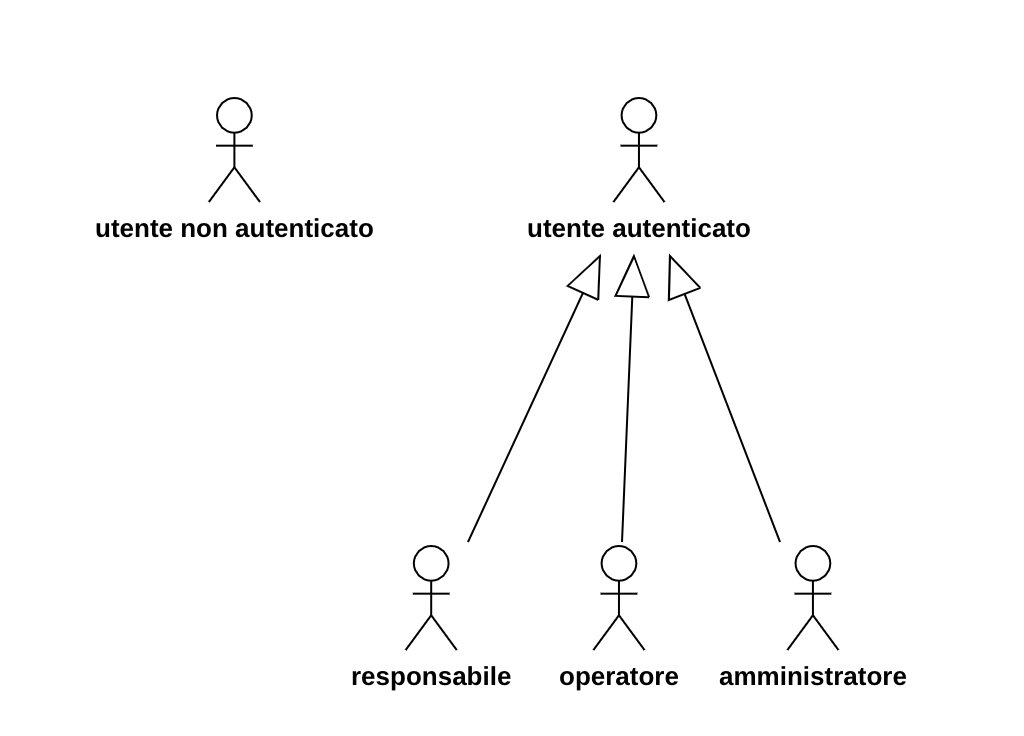
\includegraphics[scale=0.52]{res/images/gerarchia.png}
%	\caption{Attori primari}
%\end{figure}


\subsection{Diagramma di attività}

\begin{figure}[H]
	\centering
	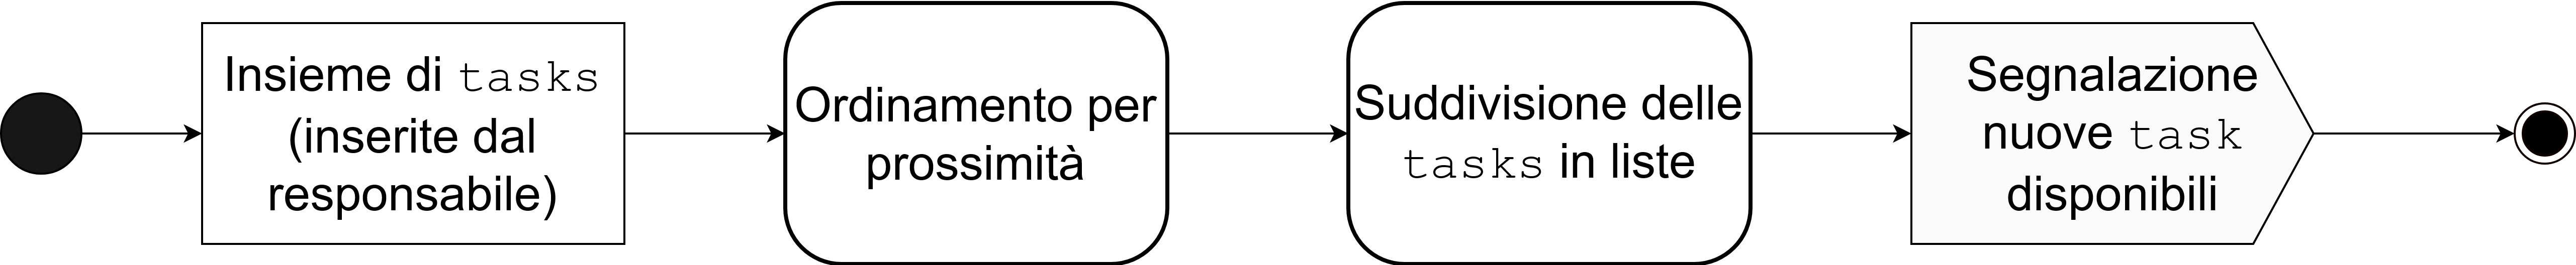
\includegraphics[scale=0.35]{res/images/diagramma_di_attivita3.png}
	\caption[Diagramma di attivita\textsubscript{G} per l'ordinamento  delle tasks]{Il diagramma mostra come le task\textsubscript{G} inserite dal responsabile vengano suddivise in liste a seconda della distanza dalla base: ogni lista sarà affidata ad un muletto per la sua esecuzione.}
\end{figure}

\begin{figure}[H]
	\centering
	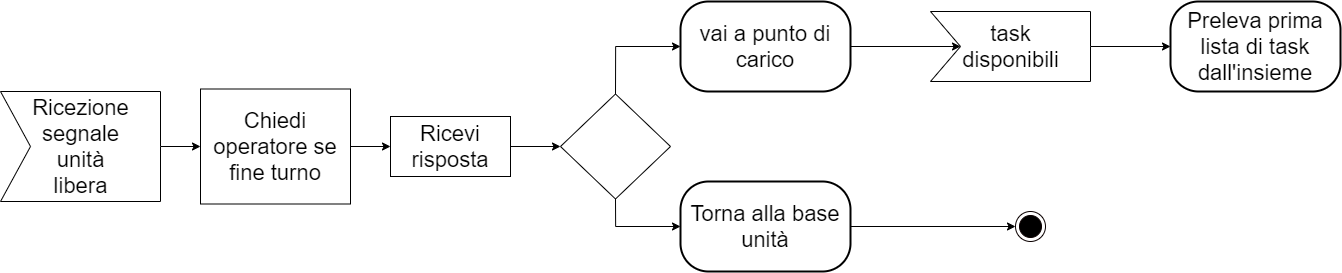
\includegraphics[scale=0.35]{res/images/diagramma_di_attivita1.png}
	\caption[Diagramma di attivita\textsubscript{G} per la gestione del muletto dopo il completamento della lista di tasks]{Completati i task\textsubscript{G}, il muletto viene riportato alla base se il turno dell'operatore è concluso, al punto di carico in caso contrario, per la presa in carico dei compiti successivi}
\end{figure}



\begin{figure}[H]
	\centering
	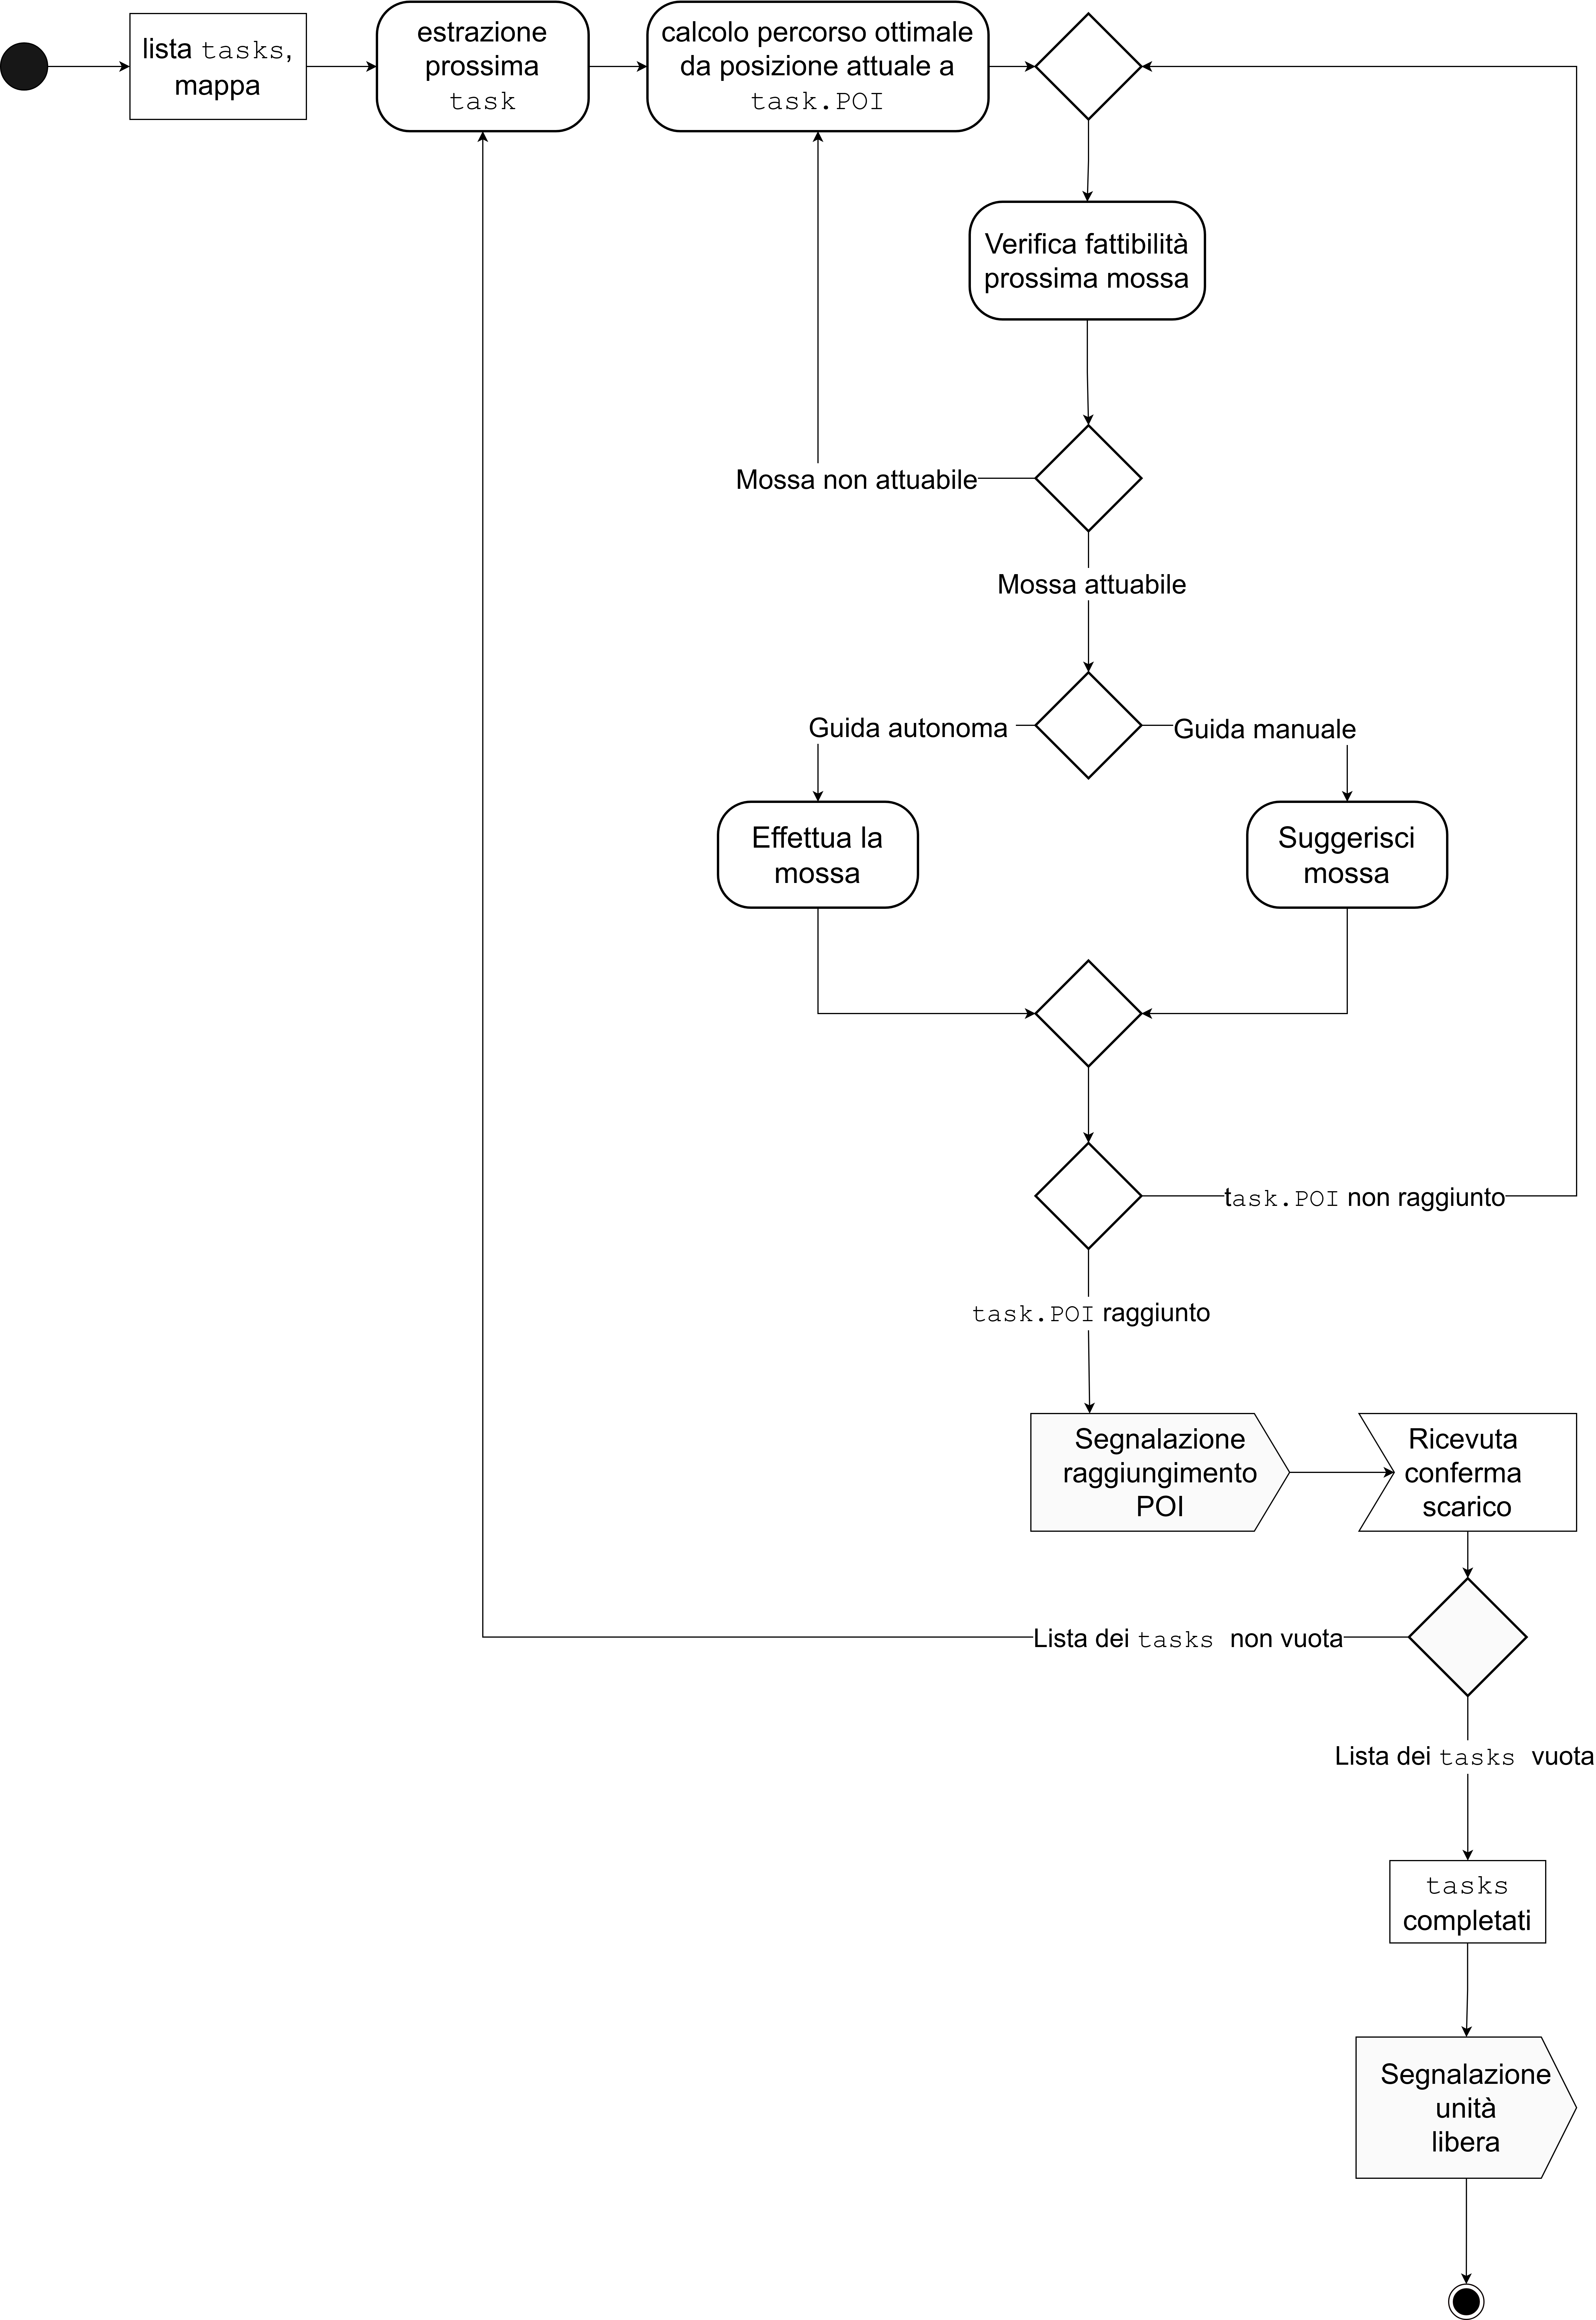
\includegraphics[scale=0.37]{res/images/diagramma_di_attivita2.png}
	\caption[Diagramma di attivita\textsubscript{G} per l'evasione di una lista di task\textsubscript{G} da parte di un muletto]{Il diagramma delinea il workflow che interessa il muletto durante l'esecuzione di una lista di task\textsubscript{G}. Il server centrale valuta la fattibilità di ogni mossa che conduce il muletto al POI\textsubscript{A} di destinazione: se la mossa non è attuabile viene ricalcolato il percorso. Al completamento di tutti i task\textsubscript{G}, l'unità viene segnalata come libera}
\end{figure}






	\pagebreak

	\section{Requisiti}
\subsection{Introduzione}
In questa sezione vengono riportati i requisito\textsubscript{G}, strutturati secondo la loro classificazione per tipologia, ovvero requisito\textsubscript{G} funzionali, requisito\textsubscript{G} prestazionali, requisito\textsubscript{G} di qualità e requisito\textsubscript{G} di vincolo.
\subsection{Requisiti funzionali}
\renewcommand{\arraystretch}{1.5}
\rowcolors{2}{pari}{dispari}
\begin{longtable}{ 
		>{}p{0.135\textwidth} 
		>{}p{0.5425\textwidth}
		>{\centering}p{0.22\textwidth} }
	\rowcolorhead
	\centering \headertitle{Codice} &
	\centering \headertitle{Descrizione} &	
	\centering \headertitle{\normalfont \textbf{Fonte}}	
	\endfirsthead	
	\endhead
RF-1-O		&	Un utente deve effettuare il login alla piattaforma tramite il suo codice identificativo	&	UC1\tabularnewline
RF-2-O		&	Il processo di login dell'utente non va a buon fine se il codice inserito non è corretto o non è presente nel sistema	&	UC1.1\tabularnewline
RF-3-O		&	L'amministratore può registrare un nuovo lavoratore all'interno del sistema	&	UC2\tabularnewline
RF-4-O		&	L'amministratore può creare l'account di un responsabile o di un operatore	&	UC2\tabularnewline
RF-4.1-O		&	La registrazione di un nuovo utente necessita del nome del lavoratore	&	UC2.1.1\tabularnewline
RF-4.2-O		&	La registrazione di un nuovo utente necessita del cognome del lavoratore	&	UC2.1.2\tabularnewline
RF-4.3-O		&	La registrazione di un nuovo utente necessita del ruolo del lavoratore (responsabile, operatore)	&	UC2.1.3\tabularnewline
RF-5-O		&	La fase\textsubscript{G} di registrazione non va a buon fine se i dati inseriti risultano già presenti nel sistema	&	UC2.3\tabularnewline
RF-6-O		&	Il sistema permette all'amministratore di gestire gli account inseriti	&	UC3\tabularnewline
RF-6.1-O		&	Il sistema permette la modifica di un utente già registrato	&	UC3.1\tabularnewline
RF-6.1.1-O	&	L'amministratore può modificare il campo nome di un account esistente	&	UC3.1.1\tabularnewline
RF-6.1.2-O	&	L'amministratore può modificare il campo cognome di un account esistente	&	UC3.1.2\tabularnewline
RF-6.1.3-O	&	L'amministratore può modificare il campo ruolo di un account esistente (responsabile, lavoratore)	&	UC3.1.3\tabularnewline
RF-6.2-O		&	Il sistema permette l'eliminazione di un utente precedentemente registrato	&	UC3.2\tabularnewline				
RF-7-O		&	Il responsabile si occupa della gestione della lista delle task\textsubscript{G}	&	UC4\tabularnewline
RF-8-O		&	Il responsabile può inserire una nuova task\textsubscript{G} 	&	UC4.1\tabularnewline
RF-8.1-O		&	Quando il responsabile inserisce una nuova task\textsubscript{G} dovrà specificare la sua priorità 	&	UC4.2\tabularnewline
RF-8.2-O		&	Quando il responsabile inserisce una nuova task\textsubscript{G} dovrà specificare il POI\textsubscript{A} a cui fa riferimento	&	UC4.3\tabularnewline
RF-8.3-O		&	Quando il responsabile conferma l'inserimento di una nuova task\textsubscript{G} e il sistema la assegna ad un'unità che la dovrà soddisfare	&	UC4.4\tabularnewline
RF-9-O		&	Il responsabile può eliminare una task\textsubscript{G} 	&	UC4.5\tabularnewline
RF-10-O		&	Il responsabile può modificare la priorità di una task\textsubscript{G} 	&	UC4.6\tabularnewline				
RF-11-O		&	Il sistema permette all'utente di fare il logout dall'applicativo	&	UC5\tabularnewline
RF-12-O		&	Il sistema abilita il logout all'amministratore in qualsiasi momento	&	UC5\tabularnewline
RF-13-O		&	Il sistema abilita il logout al responsabile in qualsiasi momento	&	UC5\tabularnewline
RF-14-O		&	Il sistema abilita il logout all'operatore solo quando si trova in base 	&	UC5\tabularnewline				
RF-15-O		&	Il sistema permette la visualizzazione della mappa all'amministratore e ai responsabili	&	UC6\tabularnewline
RF-15.1-O		&	Il sistema permette la visualizzazione di tutti i tipi di POI\textsubscript{A} nella mappa all'amministratore e ai responsabili	&	UC6\tabularnewline
RF-15.2-O		&	Il sistema permette la visualizzazione delle caratteristiche delle zone di percorrenza\textsubscript{G} (senso di marcia, numero massimo di unità che possono transitare) all'amministratore e ai responsabili	& UC6\tabularnewline
RF-15.2.1-O	&	Il sistema permette la visualizzazione delle zone non transitabili all'amministratore e ai responsabili	&	UC6 \tabularnewline
RF-16-O		&	Il sistema permette la visualizzazione della posizione dei muletti in real-time sulla mappa	&	UC6.1\tabularnewline
RF-17-F		&	Il sistema permette la visualizzazione della posizione delle persone in real-time sulla mappa	&	Capitolato\tabularnewline
RF-18-O		&	Il sistema permette all'amministratore la visualizzazione di una notifica in caso della segnalazione da parte di un operatore di un evento eccezionale	&	UC6.2\tabularnewline				
RF-19-O		&	L'amministratore autenticato può accedere all'interfaccia per gestire la mappa 	&	UC7\tabularnewline
RF-19.1-O		&	L'amministratore può modificare planimetria\textsubscript{G} del magazzino	&	UC7.2\tabularnewline
RF-19.2-O		&	L'amministratore può modificare la percorrenza\textsubscript{G} del magazzino	&	UC7.3\tabularnewline
RF-20-O		&	L'amministratore può gestire i POI\textsubscript{A}	&	UC7.4\tabularnewline
RF-20.1-O		&	L'amministratore può modificare la posizione di un POI\textsubscript{A} già esistente	&	UC7.4.1\tabularnewline
RF-20.2-O		&	L'amministratore può inserire un nuovo POI\textsubscript{A}	&	UC7.4.2\tabularnewline
RF-20.2.1-O	&	Inserendo un nuovo POI\textsubscript{A}, l'amministratore dovrà specificare la sua posizione nella mappa	&	UC7.4.3\tabularnewline
RF-20.2.2-O	&	Inserendo un nuovo POI\textsubscript{A}, l'amministratore dovrà specificare il suo codice identificativo	&	UC7.4.4\tabularnewline
RF-20.2.3-O	&	Inserendo un nuovo POI\textsubscript{A}, l'amministratore dovrà specificare il tipo di POI\textsubscript{A} inserito (carico, scarico, base)	&	UC7.4.5\tabularnewline
RF-20.3-O		&	L'amministratore può eliminare un POI\textsubscript{A}	&	UC7.4.6\tabularnewline
RF-20-O		&	La User Interface di una specifica unità attiva implementa una mappa contente i relativi POI\textsubscript{A} presenti nella lista delle task\textsubscript{G} da soddisfare, numerati secondo la lista	&	UC8.1\tabularnewline
RF-22-O		&	La User Interface implementa sotto alla mappa una lista ordinata contenente la task\textsubscript{G} rimanenti da eseguire dell'operatore che sta usando l'unità	&	UC8.2\tabularnewline
RF-23-O		&	La mappa mostra il prossimo task\textsubscript{G} da soddisfare (POI da raggiungere) 	&	UC8.3\tabularnewline
RF-23.1-O		&	Nella mappa specifica dell'unità verrà evidenziato con un colore diverso il prossimo POI\textsubscript{A} da raggiungere	&	UC8.3\tabularnewline
RF-24-O		&	L'operatore segnala al sistema la conclusione dell'incarico attraverso la User Interface	&	UC9\tabularnewline				
RF-25-O		&	La User Interface che rappresenterà ogni singola unità dovrà prevedere le 4 frecce direzionali che indicano il suggerimento del server centrale	&	UC10\tabularnewline
RF-25.1-O		&	Il sistema permette all'operatore la visualizzazione di direzione e spostamento del muletto a cui è a bordo, in caso in cui nel muletto sia attiva la guida automatica 	&	UC10\tabularnewline				
RF-26-O		&	Nella User Interface è presente un pulsante che permette di passare dalla guida manuale alla guida autonoma dell'unità	&	UC11.1\tabularnewline
RF-26.1-O		&	La User Interface del controllo manuale permette di passare alla guida autonoma	&	UC11.1, \textsc{\textsc{Verbale Esterno 1}}\tabularnewline
RF-27-O		&	Nella User Interface è presente un pulsante che permette di passare dalla guida autonoma alla guida manuale dell'unità	&	UC11.2\tabularnewline
RF-27.1-O		&	La User Interface del controllo automatico permette di passare alla guida manuale	&	UC11.2, \textsc{\textsc{Verbale Esterno 1}}\tabularnewline
RF-28-O		&	Nella User Interface è presente un pulsante che permette di segnalare al server un evento eccezionale	&	UC11.3\tabularnewline
RF-29-O		&	Nella User Interface comparirà  un pulsante per il ritorno alla base dell'unità se l'operatore avrà concluso tutte le task\textsubscript{G} assegnategli e la guida sarà impostata ad autonoma 	&	UC11.5\tabularnewline 
RF-30-O		&	La User Interface che rappresenterà ogni singola unità dovrà prevedere le 4 frecce direzionali che permettono gli spostamenti manuali ed i pulsanti di start/stop	&	UC11.4, \textsc{\textsc{Verbale Esterno 1}}\tabularnewline
RF-31-D		&	Il pannello permette di visualizzare l'indicatore di velocità attuale (che avrà come massimo la velocità massima anagrafica)	&	Capitolato\tabularnewline				
RF-32-O		&	Il server centrale pilota e coordina tutte le unità per evitare incidenti e ingorghi	&	Capitolato\tabularnewline
RF-33-F		&	Il server centrale fornisce il percorso migliore ad ogni unità tramite algoritmi di ricerca operativa	&	Capitolato\tabularnewline				
RF-34-O		&	Il sistema permette al responsabile di visualizzare la lista di tutti i POI\textsubscript{A} con il proprio tipo (carico, scarico, base) presenti nella mappa	&	UC12\tabularnewline
RF-35-O		&	Il sistema permette all'amministratore di visualizzare la lista di tutti i POI\textsubscript{A} con il proprio tipo (carico, scarico, base) presenti nella mappa	&	UC12\tabularnewline				
RF-36-O		&	Il responsabile ha a disposizione un pulsante per poter vedere una lista completa delle task\textsubscript{G}	&	UC13\tabularnewline			
RF-37-O		&	L'amministratore ha a disposizione un'interfaccia su cui può gestire le unità	&	UC14\tabularnewline
RF-37.1-O		&	L'amministratore può aggiungere una nuova unità	&	UC14.1\tabularnewline
RF-37.2-O		&	L'amministratore può eliminare un'unità	&	UC14.2\tabularnewline
\caption{Tabella Requisiti Funzionali\label{ Tabella Requisiti Funzionali}}
\end{longtable}.
\subsection{Requisiti prestazionali}
In questo progetto\textsubscript{G} non sono stati rilevati alcuni requisito\textsubscript{G} prestazionali per quanto riguarda i requisito\textsubscript{G} obbligatori.
\subsection{Requisiti di qualità}
\renewcommand{\arraystretch}{1.5}
\rowcolors{2}{pari}{dispari}
\begin{longtable}{ 
		>{}p{0.135\textwidth} 
		>{}p{0.5425\textwidth}
		>{\centering}p{0.2\textwidth} }
	\rowcolorhead
	\centering\headertitle{Codice} &
	\centering \headertitle{Descrizione} &	
	\centering \headertitle{\normalfont \textbf{Fonte}}	
	\endfirsthead	
	\endhead
RQ-1-O & Disporre di diagrammi UML\textsubscript{A} relativi agli use cases di progetto\textsubscript{G} & Capitolato\tabularnewline
RQ-2-O & Disporre di uno schema design relativo alla base dati (se ritenuta necessaria) & Capitolato\tabularnewline
RQ-3-O & Rendere disponibile la documentazione delle API\textsubscript{A} che saranno realizzate & Capitolato\tabularnewline
RQ-4-O & Rendere disponibile la lista dei bug\textsubscript{G} risolti durante la fase\textsubscript{G} di sviluppo & Capitolato\tabularnewline
RQ-5-O & Fornire il codice prodotto in formato sorgente utilizzando sistemi di versionamento del codice, quali GitHub o Bitbucket & Capitolato\tabularnewline
RQ-6-O & Rilasciare il codice sorgente di quanto realizzato & Capitolato\tabularnewline
RQ-7-O & Rendere disponibile il Docker file (\#1) con la componente applicativa, rappresentante il motore di calcolo & Capitolato\tabularnewline 
RQ-8-O & Fornire il Docker file (\#2) con la componente applicativa rappresentante il visualizzatore/monitor real-time (in base all'implementazione, potrebbe essere incorporato nel \#1) & Capitolato\tabularnewline
RQ-9-O & Erogare il Docker file (\#3), da istanziare N volte, rappresentante la singola unità & Capitolato\tabularnewline
RQ-10-F & Rendere disponibile il Docker file (\#4), da istanziare N volte, rappresentante il singolo pedone & Capitolato\tabularnewline 
\caption{Tabella Requisiti di Qualità\label{ Tabella Requisiti di Qualità}}
\end{longtable}.
\newline 
\subsection{Requisiti di vincolo}
\renewcommand{\arraystretch}{1.5}
\rowcolors{2}{pari}{dispari}
\begin{longtable}{ 
		>{}p{0.135\textwidth} 
		>{}p{0.5425\textwidth}
		>{\centering}p{0.2\textwidth} }
	\rowcolorhead
	\centering\headertitle{Codice} &
	\centering \headertitle{Descrizione} &	
	\centering \headertitle{\normalfont \textbf{Fonte}}	
	\endfirsthead	
	\endhead
RV-1-O & La geolocalizzazione va simulata & Capitolato\tabularnewline
RV-2-O & L'applicativo propone una mappatura in tempo reale della posizione georeferenziata delle unità & Capitolato\tabularnewline
RV-3-F & L'applicativo propone una mappatura in tempo reale della posizione georeferenziata delle persone & Capitolato\tabularnewline
RV-4-O & Le persone si muovano solo a bordo di mezzi & Decisione interna\tabularnewline
RV-5-O & Il server centrale deve prevedere ed evitare le collisioni & Capitolato\tabularnewline
RV-6-O & Ogni zona di percorrenza\textsubscript{G} ha un numero massimo di unità che possono percorrerla contemporaneamente (dimensione della zona) & Capitolato\tabularnewline
RV-7-O & Ogni zona di percorrenza\textsubscript{G} ha un modo in cui può essere percorsa (senso unico, doppio senso) & Capitolato\tabularnewline
RV-8-O & Ogni unità deve rispettare i vincoli dimensionali delle zone & Capitolato\tabularnewline
RV-9-O & Tutte le unità, quando sono in movimento, viaggiano alla stessa velocità che rimane costante & Capitolato\tabularnewline
RV-10-F & L'applicativo permette di gestire il cambiamento della velocità di un'unità & Capitolato\tabularnewline
RV-11-D & Ogni unità ha una velocità di crociera & Capitolato\tabularnewline
RV-12-D & Ogni unità ha una velocità massima & Capitolato\tabularnewline
RV-13-O & Ogni unità ha un suo identificativo & Capitolato\tabularnewline
RV-14-O & Il server centrale conosce la posizione di ogni singola unità & Capitolato\tabularnewline
RV-15-O & Il server centrale centrale conosce la direzione di ogni singola unità & Capitolato\tabularnewline
RV-16-D & Il server centrale conosce la velocità di ogni singola unità & Capitolato\tabularnewline
RV-17-O & Ogni unità ha una lista di task\textsubscript{G} da risolvere ogni volta che fa carico & Capitolato\tabularnewline
RV-18-O & Ogni task\textsubscript{G} è collegata ad un POI\textsubscript{A} da raggiungere & Capitolato\tabularnewline
RV-19-O & Ogni POI\textsubscript{A} può essere di carico o scarico o base & Decisione interna\tabularnewline
RV-20-O & Ci devono essere più di un POI\textsubscript{A} di scarico & Decisione interna\tabularnewline
RV-21-O & Ci deve essere almeno un POI\textsubscript{A} di base & Decisione interna\tabularnewline
RV-22-O & Ci deve essere almeno un POI\textsubscript{A} di carico & Decisione interna\tabularnewline
RV-23-F & Ci possono essere più POI\textsubscript{A} di base & Decisione interna\tabularnewline
RV-24-F & Ci possono essere più POI\textsubscript{A} di carico & Decisione interna\tabularnewline
RV-25-O & Ogni unità parte da una base. La sua partenza dalla base determina l'inizio del turno di un operatore & Decisione interna\tabularnewline
RV-26-O & Ogni unità torna ad una base quando termina il turno dell'operatore & Decisione interna\tabularnewline
RV-27-O & Ogni unità passa per un'area di carico prima di iniziare la sequenza di scarichi (tasks) & Decisione interna\tabularnewline
RV-28-O & Ogni unità torna ad un'area di carico se ha scaricato tutta la merce (completato i task) e il turno dell'operatore non è terminato & Decisione interna\tabularnewline
RV-29-O & Il server centrale conosce ogni spostamento (in avanti, indietro, a destra e a sinistra) di ogni unità & Capitolato\tabularnewline
RV-30-O & Il server centrale recepisce la fermata di ogni unità & Capitolato\tabularnewline
RV-31-O & Il server centrale recepisce la partenza di ogni unità & Capitolato\tabularnewline
RV-32-O	&	Ci deve uno e un solo account registrato con il ruolo di amministratore	&	Decisione interna	\tabularnewline
RV-33-O	&	Ci deve essere almeno un account registrato con il ruolo di responsabile	&	Decisione interna	\tabularnewline
RV-34-F	&	Ci possono essere più account registrati con il ruolo di responsabile	&	Decisione interna	\tabularnewline
RV-35-O	&	Ci devono essere più account registrati con il ruolo di operatore	&	Decisione interna	\tabularnewline
\caption{Tabella Requisiti di vincolo\label{ Tabella Requisiti di vincolo}}
\end{longtable}.
\pagebreak
\subsection{Tracciamento}
\subsubsection{Fonti - Requisiti}
\renewcommand{\arraystretch}{1.5}
\rowcolors{2}{pari}{dispari}
\begin{longtable}{ 
		>{}p{0.22\textwidth} 
		>{}p{0.25\textwidth} }
	\rowcolorhead
	\headertitle{Fonte} &
	\headertitle{\normalfont \textbf{Requisiti}}	
	\endfirsthead	
	\endhead
Capitolato &	
	RV-1-O	\newline
	RV-2-O	\newline
	RV-3-F	\newline
	RV-5-O	\newline
	RV-6-O	\newline
	RV-7-O	\newline
	RV-8-O	\newline
	RV-9-O	\newline
	RV-10-F	\newline
	RV-11-D	\newline
	RV-12-D	\newline
	RV-13-O	\newline
	RV-14-O	\newline
	RV-15-O	\newline
	RV-16-D	\newline
	RV-17-O	\newline
	RV-18-O	\newline
	RV-29-O	\newline
	RV-30-O	\newline
	RV-31-O	\newline
	RF-17-F	\newline
	RF-31-D	\newline
	RF-32-O	\newline
	RF-33-F	\newline
	RQ-1-O	\newline
	RQ-2-O	\newline
	RQ-3-O	\newline
	RQ-4-O	\newline
	RQ-5-O	\newline
	RQ-6-O	\newline
	RQ-7-O	\newline
	RQ-8-O	\newline
	RQ-9-O	\newline
	RQ-10-F	\tabularnewline
Decisione interna &	RV-4-O	\newline
	RV-19-O	\newline
	RV-20-O	\newline
	RV-21-O	\newline
	RV-22-O	\newline
	RV-23-F	\newline
	RV-24-F	\newline
	RV-25-O	\newline
	RV-26-O	\newline
	RV-27-O	\newline
	RV-28-O	\newline
	RV-32-O	\newline
	RV-33-O	\newline
	RV-34-O	\newline
	RV-35-O	\tabularnewline
\textsc{Verbale Esterno 1} &	RF-26.1-O	\newline
	RF-27.1-O	\newline
	RF-30-O	\tabularnewline
UC1 &	RF-1-O	\newline
	RF-2-O	\tabularnewline
UC2 &	RF-3-O	\newline
	RF-4-O	\newline
	RF-4.1-O	\newline
	RF-4.2-O	\newline
	RF-4.3-O	\newline
	RF-5-O	\tabularnewline
UC3 &	RF-6-O	\newline
	RF-6.1-O	\newline
	RF-6.1.1-O	\newline
	RF-6.1.2-O	\newline
	RF-6.1.3-O	\newline
	RF-6.2-O	\tabularnewline
UC4 &	RF-7-O	\newline
	RF-8-O	\newline
	RF-8.1-O	\newline
	RF-8.2-O	\newline
	RF-8.3-O	\newline
	RF-9-O	\newline
	RF-10-O	\tabularnewline
UC5 &	RF-11-O	\newline
	RF-12-O	\newline
	RF-13-O	\newline
	RF-14-O	\tabularnewline
UC6 &	RF-15-O	\newline
	RF-15.1-O	\newline
	RF-15.2-O	\newline
	RF-15.2.1-O	\newline
	RF-16-O	\newline
	RF-18-O	\tabularnewline
UC7 &	RF-19-O	\newline
	RF-19.1-O	\newline
	RF-19.2-O	\newline
	RF-20-O	\newline
	RF-20.1-O	\newline
	RF-20.2-O	\newline
	RF-20.2.1-O	\newline
	RF-20.2.2-O	\newline
	RF-20.2.3-O	\newline
	RF-20.3-O	\tabularnewline
UC8 &	RF-20-O	\newline
	RF-22-O	\newline
	RF-23-O	\newline
	RF-23.1-O	\tabularnewline
UC9 &	RF-24-O	\tabularnewline
UC10 &	RF-25-O	\newline
	RF-25.1-O	\tabularnewline
UC11 &	RF-26-O	\newline
	RF-26.1-O	\newline
	RF-27-O	\newline
	RF-27.1-O	\newline
	RF-28-O	\newline
	RF-29-O	\newline
	RF-30-O	\tabularnewline
UC12 &	RF-34-O	\newline
	RF-35-O	\tabularnewline
UC13 &	RF-36-O	\tabularnewline
UC14 &	RF-37-O	\newline
	RF-37.1-O	\newline
	RF-37.2-O	\tabularnewline
\caption{Tabella Fonti - Requisiti\label{ Tabella Fonti - Requisiti}}
\end{longtable}.
\pagebreak
\subsubsection{Requisiti - Fonti}
\renewcommand{\arraystretch}{1.5}
\rowcolors{2}{pari}{dispari}
\begin{longtable}{ 
		>{}p{0.2\textwidth} 
		>{}p{0.35\textwidth} }
	\rowcolorhead
	\headertitle{Requisito} &
	\headertitle{\normalfont \textbf{Fonti}}	
	\endfirsthead	
	\endhead
RF-1-O	&	UC1	\tabularnewline
RF-2-O	&	UC1.1	\tabularnewline
RF-3-O	&	UC2	\tabularnewline
RF-4-O	&	UC2	\tabularnewline
RF-4.1-O	&	UC2.1.1	\tabularnewline
RF-4.2-O	&	UC2.1.2	\tabularnewline
RF-4.3-O	&	UC2.1.3	\tabularnewline
RF-5-O	&	UC2.3	\tabularnewline
RF-6-O	&	UC3	\tabularnewline
RF-6.1-O	&	UC3.1	\tabularnewline
RF-6.1.1-O	&	UC3.1.1	\tabularnewline
RF-6.1.2-O	&	UC3.1.2	\tabularnewline
RF-6.1.3-O	&	UC3.1.3	\tabularnewline
RF-6.2-O	&	UC3.2	\tabularnewline
RF-7-O	&	UC4	\tabularnewline
RF-8-O	&	UC4.1	\tabularnewline
RF-8.1-O	&	UC4.2	\tabularnewline
RF-8.2-O	&	UC4.3	\tabularnewline
RF-8.3-O	&	UC4.4	\tabularnewline
RF-9-O	&	UC4.5	\tabularnewline
RF-10-O	&	UC4.6	\tabularnewline
RF-11-O	&	UC5	\tabularnewline
RF-12-O	&	UC5	\tabularnewline
RF-13-O	&	UC5	\tabularnewline
RF-14-O	&	UC5	\tabularnewline
RF-15-O	&	UC6	\tabularnewline
RF-15.1-O	&		\tabularnewline
RF-15.2-O	&	UC6	\tabularnewline
RF-15.2.1-O	&	UC6	\tabularnewline
RF-16-O	&	UC6.1	\tabularnewline
RF-17-F	&	Capitolato	\tabularnewline
RF-18-O	&	UC6.2	\tabularnewline
RF-19-O	&	UC7	\tabularnewline
RF-19.1-O	&	UC7.2	\tabularnewline
RF-19.2-O	&	UC7.3	\tabularnewline
RF-20-O	&	UC7.4	\tabularnewline
RF-20.1-O	&	UC7.4.1	\tabularnewline
RF-20.2-O	&	UC7.4.2	\tabularnewline
RF-20.2.1-O	&	UC7.4.3	\tabularnewline
RF-20.2.2-O	&	UC7.4.4	\tabularnewline
RF-20.2.3-O	&	UC7.4.5	\tabularnewline
RF-20.3-O	&	UC7.4.6	\tabularnewline
RF-20-O	&	UC8.1	\tabularnewline
RF-22-O	&	UC8.2	\tabularnewline
RF-23-O	&	UC8.3	\tabularnewline
RF-23.1-O	&	UC8.3	\tabularnewline
RF-24-O	&	UC9	\tabularnewline
RF-25-O	&	UC10	\tabularnewline
RF-25.1-O	&	UC10	\tabularnewline
RF-26-O	&	UC11.1	\tabularnewline
RF-26.1-O	&	UC11.1, \textsc{Verbale Esterno 1}	\tabularnewline
RF-27-O	&	UC11.2	\tabularnewline
RF-27.1-O	&	UC11.2, \textsc{Verbale Esterno 1}	\tabularnewline
RF-28-O	&	UC11.3	\tabularnewline
RF-29-O	&	UC11.5	\tabularnewline
RF-30-O	&	UC11.4, \textsc{Verbale Esterno 1}	\tabularnewline
RF-31-D	&	Capitolato	\tabularnewline
RF-32-O	&	Capitolato	\tabularnewline
RF-33-F	&	Capitolato	\tabularnewline
RF-34-O	&	UC12	\tabularnewline
RF-35-O	&	UC12	\tabularnewline
RF-36-O	&	UC13	\tabularnewline
RF-37-O	&	UC14	\tabularnewline
RF-37.1-O	&	UC14.1	\tabularnewline
RF-37.2-O	&	UC14.2	\tabularnewline
RQ-1-O	&	Capitolato	\tabularnewline
RQ-2-O	&	Capitolato	\tabularnewline
RQ-3-O	&	Capitolato	\tabularnewline
RQ-4-O	&	Capitolato	\tabularnewline
RQ-5-O	&	Capitolato	\tabularnewline
RQ-6-O	&	Capitolato	\tabularnewline
RQ-7-O	&	Capitolato	\tabularnewline
RQ-8-O	&	Capitolato	\tabularnewline
RQ-9-O	&	Capitolato	\tabularnewline
RQ-10-F	&	Capitolato	\tabularnewline
RV-1-O	&	Capitolato	\tabularnewline
RV-2-O	&	Capitolato	\tabularnewline
RV-3-F	&	Capitolato	\tabularnewline
RV-4-O	&	Decisione interna	\tabularnewline
RV-5-O	&	Capitolato	\tabularnewline
RV-6-O	&	Capitolato	\tabularnewline
RV-7-O	&	Capitolato	\tabularnewline
RV-8-O	&	Capitolato	\tabularnewline
RV-9-O	&	Capitolato	\tabularnewline
RV-10-F	&	Capitolato	\tabularnewline
RV-11-D	&	Capitolato	\tabularnewline
RV-12-D	&	Capitolato	\tabularnewline
RV-13-O	&	Capitolato	\tabularnewline
RV-14-O	&	Capitolato	\tabularnewline
RV-15-O	&	Capitolato	\tabularnewline
RV-16-D	&	Capitolato	\tabularnewline
RV-17-O	&	Capitolato	\tabularnewline
RV-18-O	&	Capitolato	\tabularnewline
RV-19-O	&	Decisione interna	\tabularnewline
RV-20-O	&	Decisione interna	\tabularnewline
RV-21-O	&	Decisione interna	\tabularnewline
RV-22-O	&	Decisione interna	\tabularnewline
RV-23-F	&	Decisione interna	\tabularnewline
RV-24-F	&	Decisione interna	\tabularnewline
RV-25-O	&	Decisione interna	\tabularnewline
RV-26-O	&	Decisione interna	\tabularnewline
RV-27-O	&	Decisione interna	\tabularnewline
RV-28-O	&	Decisione interna	\tabularnewline
RV-29-O	&	Capitolato	\tabularnewline
RV-30-O	&	Capitolato	\tabularnewline
RV-31-O	&	Capitolato	\tabularnewline
RV-32-O	&	Decisione interna	\tabularnewline
RV-33-O	&	Decisione interna	\tabularnewline
RV-34-F	&	Decisione interna	\tabularnewline
RV-35-O	&	Decisione interna	\tabularnewline
\caption{Tabella Requisiti - Fonti\label{ Tabella Requisiti - Fonti}}
\end{longtable}.
\subsubsection{Riepilogo requisiti}
\renewcommand{\arraystretch}{1.5}
\rowcolors{2}{pari}{dispari}
\begin{longtable}{ 
		>{\centering}p{0.15\textwidth} 
		>{\centering}p{0.15\textwidth}
		>{\centering}p{0.15\textwidth}
		>{\centering}p{0.15\textwidth}
		>{\centering}p{0.1\textwidth} }
	\rowcolorhead
	\headertitle{Tipologia} &
	\centering \headertitle{Obbligatorio} &	
	\centering \headertitle{Facoltativo} &	
	\centering \headertitle{Desiderabile} &	
	\headertitle{\normalfont \textbf{Totale}}	
	\endfirsthead	
	\endhead
Funzionale & 62 & 2 & 1 & 65\tabularnewline
Di Qualità & 9 & 1 & 0 & 10\tabularnewline
Di Vincolo & 27 & 5 & 3 & 35\tabularnewline
\caption{Tabella Riepilogo dei Requisiti\label{ Tabella Riepilogo dei Requisiti}}
\end{longtable}.

	\pagebreak
	
	\printglossary[type=\acronymtype,title=Lista degli Acronimi]
	\printglossary[title=Glossario dei Termini]	
	
\end{document}
